% Pengaturan ukuran teks dan bentuk halaman dua sisi
\documentclass[12pt]{book}

% Pengaturan ukuran halaman dan margin
\usepackage[a4paper,top=30mm,left=30mm,right=20mm,bottom=25mm]{geometry}

% Pengaturan ukuran spasi
\usepackage[singlespacing]{setspace}

% Pengaturan caption untuk tabel
\usepackage{caption}

% Judul dokumen
\title{Proposal Tugas Akhir ITS}
\author{Musk, Elon Reeve}

% Pengaturan detail pada file PDF
\usepackage[pdfauthor={\@author},bookmarksnumbered,pdfborder={0 0 0}]{hyperref}


% Pengaturan ukuran indentasi
\setlength{\parindent}{2em}

% Package lainnya
\usepackage{changepage}
\usepackage{etoolbox} % Mengubah fungsi default

% Pengaturan jenis karakter
\usepackage[utf8]{inputenc}

\usepackage[style=ieee, backend=biber]{biblatex}
\usepackage{enumitem} % Pembuatan list
\usepackage{lipsum} % Pembuatan template kalimat
\usepackage{graphicx} % Input gambar
\usepackage{longtable} % Pembuatan tabel
\usepackage[table,xcdraw]{xcolor} % Pewarnaan tabel
\usepackage{eso-pic} % Untuk menggunakan background image di halaman
\usepackage{txfonts} % Font times
\usepackage{changepage} % Pembuatan teks kolom
\usepackage{multicol} % Pembuatan kolom ganda
\usepackage{multirow} % Pembuatan baris ganda
\usepackage{tabularx} % Untuk mengatur kolom, seperti grid pada CSS
\usepackage{wrapfig}
\usepackage{float}

% Pengaturan format daftar isi, daftar gambar, dan daftar tabel
\usepackage[titles]{tocloft}
\setlength{\cftsecindent}{2em}
\setlength{\cftsubsecindent}{2em}
\setlength{\cftbeforechapskip}{1.5ex}
\setlength{\cftbeforesecskip}{1.5ex}
\setlength{\cftbeforetoctitleskip}{0cm}
\setlength{\cftbeforeloftitleskip}{0cm}
\setlength{\cftbeforelottitleskip}{0cm}
\renewcommand{\cfttoctitlefont}{\hfill\Large\bfseries} % command untuk membuat heading bold dan besar
\renewcommand{\cftaftertoctitle}{\hfill}
\renewcommand{\cftloftitlefont}{\hfill\Large\bfseries}
\renewcommand{\cftafterloftitle}{\hfill}
\renewcommand{\cftlottitlefont}{\hfill\Large\bfseries}
\renewcommand{\cftafterlottitle}{\hfill}

% Definisi untuk "Hati ini sengaja dikosongkan"
\patchcmd{\cleardoublepage}{\hbox{}}{
  \thispagestyle{empty}
  \vspace*{\fill}
  \begin{center}\textit{[Halaman ini sengaja dikosongkan]}\end{center}
  \vfill}{}{}

  % Pengaturan penomoran halaman
\usepackage{fancyhdr}
\fancyhf{}
\renewcommand{\headrulewidth}{0pt}
\pagestyle{fancy}
\fancyfoot[C,CO]{\thepage}
\patchcmd{\chapter}{plain}{fancy}{}{}
\patchcmd{\chapter}{empty}{plain}{}{}

% Pengaturan format judul bab
\usepackage{titlesec}
\renewcommand{\thesection}{\thechapter.\arabic{section}}
\titleformat{\chapter}[hang]{\centering\bfseries\large}{BAB\ \arabic{chapter}\ }{0ex}{\vspace{0ex}\centering}
\titleformat*{\section}{\large\bfseries}
\titleformat*{\subsection}{\normalsize\bfseries}
\titlespacing{\chapter}{0ex}{0ex}{4ex}
\titlespacing{\section}{0ex}{1ex}{0ex}
\titlespacing{\subsection}{0ex}{0.5ex}{0ex}
\titlespacing{\subsubsection}{0ex}{0.5ex}{0ex}
\setcounter{secnumdepth}{3} % Untuk memberi penomoran pada \subsubsection

\counterwithin{figure}{chapter}
\counterwithin{table}{chapter}

% Mengganti figure dan table menjadi gambar dan tabel
\renewcommand{\figurename}{Gambar}
\renewcommand{\tablename}{Tabel}

% Tambahkan format tanda hubung yang benar di sini
\hyphenation{
  ro-ket
  me-ngem-bang-kan
  per-hi-tu-ngan
}

% Menambahkan resource daftar pustaka
\addbibresource{pustaka/pustaka.bib}
\tolerance=9999
\emergencystretch=10pt
\hyphenpenalty=10000
\exhyphenpenalty=100
% Isi keseluruhan dokumen
\begin{document}
  % Nomor halaman pembuka dimulai dari sini
  \pagenumbering{roman}

  % Atur ulang penomoran halaman
  \setcounter{page}{1}

  % Sampul Bahasa Indonesia
  \newcommand\covercontents{sampul/konten-id.tex}
  \AddToShipoutPictureBG*{
  \AtPageLowerLeft{
    % Ubah nilai berikut jika posisi horizontal background tidak sesuai
    \hspace{-3.25mm}

    % Ubah nilai berikut jika posisi vertikal background tidak sesuai
    \raisebox{0mm}{
      
\includegraphics[width=\paperwidth,height=\paperheight]{sampul/gambar/sampul-luar-tipis.png}
    }
  }
}

% Menyembunyikan nomor halaman
\thispagestyle{empty}

% Pengaturan margin untuk menyesuaikan konten sampul
\newgeometry{
  top=65mm,
  left=30mm,
  right=30mm,
  bottom=20mm
}

\begin{flushleft}

  % Pemilihan font sans serif
  \sffamily

  % Pemilihan font bold
  \fontseries{bx}
  \selectfont
  \begin{spacing}{1.5}
    \input{\covercontents}
  \end{spacing}

\end{flushleft}

\restoregeometry


  % Lembar pengesahan
  \chapter*{LEMBAR PENGESAHAN}

% Menyembunyikan nomor halaman
\thispagestyle{empty}

\begin{center}
  % Ubah kalimat berikut dengan judul tugas akhir
  \textbf{SISTEM KENDALI KURSI RODA ELEKTRIK MENGGUNAKAN \textit{TOUCHPAD} BERBASIS \textit{RASPBERRY PI}}
\end{center}

\begingroup
% Pemilihan font ukuran small
\small

\begin{center}
  % Ubah kalimat berikut dengan pernyataan untuk lembar pengesahan
  \textbf{PROPOSAL TUGAS AKHIR} \\
  Diajukan untuk memenuhi salah satu syarat memperoleh gelar
  Sarjana Teknik pada
  Program Studi S-1 Teknik Komputer \\
  Departemen Teknik Komputer \\
  Fakultas Teknologi Elektro dan Informatika Cerdas \\
  Institut Teknologi Sepuluh Nopember
\end{center}

\begin{center}
  % Ubah kalimat berikut dengan nama dan NRP mahasiswa
  Oleh: \textbf{Faruq Putra Rahardjo} \\
  NRP. 5024 20 1049
\end{center}

\begin{center}
  Disetujui Oleh:
\end{center}

\vspace{10ex}

\begingroup
% Menghilangkan padding
\setlength{\tabcolsep}{0pt}

\noindent
\begin{tabularx}{\textwidth}{X c}
  % Ubah kalimat-kalimat berikut dengan nama dan NIP dosen pembimbing pertama
  Eko Pramunanto, S.T., M.T..      &                 \\
  NIP: 19661203 199412 1 001    & (Pembimbing)    \\
                                &                 \\
                                &                 \\
                                &                 \\
  % Ubah kalimat-kalimat berikut dengan nama dan NIP dosen pembimbing kedua
  % Dosen, S.T., M.Sc. &                 \\
  % NIP: 19230323 197706 1 001    & (Ko-Pembimbing) \\
\end{tabularx}
\endgroup

\vspace{\fill}

\begin{center}
  % Ubah text dibawah menjadi tempat dan tanggal
  \textbf{SURABAYA} \\
  \textbf{Desember, 2023}
\end{center}
\endgroup

  \cleardoublepage

  \begin{center}
	\large
  \textbf{APPROVAL SHEET}
\end{center}

% Menyembunyikan nomor halaman
\thispagestyle{empty}

\begin{center}
  % Ubah kalimat berikut dengan judul tugas akhir
  \textbf{Electric Wheelchair Control System Using Touchpad Based on Raspberry Pi}
\end{center}

\begingroup
  % Pemilihan font ukuran small
  \small

  \begin{center}
    % Ubah kalimat berikut dengan pernyataan untuk lembar pengesahan
    \textbf{FINAL PROJECT PROPOSAL} \\
    Submitted to fulfill one of the requirements for obtaining a degree
    Bachelor of Engineering at 
    Undergraduate Study Program of Computer Engineering \\
    Department of Computer Engineering \\
    Faculty of Intelligent Electrical and Informatics Technology \\
    Sepuluh Nopember Institute of Technology
  \end{center}

  \begin{center}
    % Ubah kalimat berikut dengan nama dan NRP mahasiswa
    By: \textbf{Faruq Putra Rahardjo} \\
    NRP. 5024 20 1049
  \end{center}

  \begin{center}
    Approved by Final Project Proposal Examiner Team:
  \end{center}

  \begingroup
    % Menghilangkan padding
    \setlength{\tabcolsep}{0pt}

    \noindent
    \begin{tabularx}{\textwidth}{X c}
      % Ubah kalimat-kalimat berikut dengan nama dan NIP dosen pembimbing pertama
      Eko Pramunanto, S.T., M.T..          & (Advisor) \\
      NIP: 19661203 199412 1 001        & \\
      &  \\
      &  \\
      % Ubah kalimat-kalimat berikut dengan nama dan NIP dosen pembimbing kedua
      % Wernher von Braun, S.T., M.T.     & (Co-Advisor) \\
      % NIP: 19230323 197706 1 001        & \\
      % &  \\
      % &  \\
      % Ubah kalimat-kalimat berikut dengan nama dan NIP dosen penguji pertama
      % Dr. Galileo Galilei, S.T., M.Sc.  & (Examiner I) \\
      % NIP: 15640215 164201 1 001        & \\
      % &  \\
      % &  \\
      % Ubah kalimat-kalimat berikut dengan nama dan NIP dosen penguji kedua
      % Friedrich Nietzsche, S.T., M.Sc.  & (Examiner II) \\
      % NIP: 18441015 190008 1 001        & \\
      % &  \\
      % &  \\
      % Ubah kalimat-kalimat berikut dengan nama dan NIP dosen penguji ketiga
      % Alan Turing, ST., MT.             & (Examiner III) \\
      % NIP: 19120623 195406 1 001        & \\
    \end{tabularx}
  \endgroup

  \vspace{\fill}

  \begin{center}
    % Ubah text dibawah menjadi tempat dan tanggal
    \textbf{SURABAYA} \\
    \textbf{December, 2023}
  \end{center}
\endgroup

  \cleardoublepage

  % Abstrak
  \chapter*{ABSTRAK}
\begin{center}
  \large
  \textbf{SISTEM KENDALI KURSI RODA ELEKTRIK MENGGUNAKAN \textit{TOUCHPAD} BERBASIS \textit{RASPBERRY PI}}
\end{center}
\addcontentsline{toc}{chapter}{ABSTRAK}
% Menyembunyikan nomor halaman
\thispagestyle{empty}

\begin{flushleft}
  \setlength{\tabcolsep}{0pt}
  \bfseries
  \begin{tabular}{ll@{\hspace{6pt}}l}
  Nama Mahasiswa / NRP&:& Faruq Putra Rahardjo / 5024201049\\
  Departemen&:& Teknik Komputer FTEIC - ITS\\
  Dosen Pembimbing&:& 1. Eko Pramunanto, S.T., M.T.\\
  % & & 2. Dosen, S.T., M.Sc.\\
  \end{tabular}
  \vspace{4ex}
\end{flushleft}
\textbf{Abstrak}

% Isi Abstrak
Proposal  tugas akhir "Sistem Kendali Kursi Roda Elektrik Menggunakan Touchpad Berbasis Raspberry Pi" oleh Faruq Putra Rahardjo mengeksplorasi pengembangan sistem kendali berbasis touchpad untuk kursi roda elektrik menggunakan Raspberry Pi. Penelitian ini bertujuan untuk meningkatkan kemudahan operasi bagi pengguna dengan kebutuhan khusus, mempermudah mereka dalam mengoperasikan kursi roda elektrik. Sistem yang diusulkan bertujuan menggantikan kontrol joystick konvensional dengan sistem touchpad, yang diharapkan dapat meningkatkan navigasi, keamanan, dan kenyamanan bagi pengguna kursi roda. Studi ini berfokus pada integrasi teknologi touchpad dengan kontrol kursi roda, menekankan potensi untuk meningkatkan kemandirian pengguna dan kelayakan komersial industri terkait.

\vspace{2ex}
\noindent
\textbf{Kata Kunci: \emph{Kursi Roda Elektrik, Raspberry Pi, Touchpad }}
  \cleardoublepage
  
  \chapter*{ABSTRACT}
\begin{center}
  \large
  \textbf{ELECTRIC WHEELCHAIR CONTROL SYSTEM USING TOUCHPAD BASED ON RASPBERRY PI}
\end{center}
% Menyembunyikan nomor halaman
\thispagestyle{empty}

\begin{flushleft}
  \setlength{\tabcolsep}{0pt}
  \bfseries
  \begin{tabular}{lc@{\hspace{6pt}}l}
  Student Name / NRP&: &Faruq Putra Rahardjo / 5024201049\\
  Department&: &Computer Engineering FTEIC - ITS\\
  Advisor&: &1. Eko Pramunanto, S.T., M.T.\\
  % & & 2. Dosen, S.T., M.Sc.\\
  \end{tabular}
  \vspace{4ex}
\end{flushleft}
\textbf{Abstract}

% Isi Abstrak
The final project proposal titled "Electric Wheelchair Control System Using Touchpad Based on Raspberry Pi" explores the development of a touchpad-based control system for electric wheelchairs using Raspberry Pi. This research aims to improve the ease of operation for users with special needs, making it simpler for them to navigate electric wheelchairs. The proposed system seeks to replace the conventional joystick control with a touchpad system, expected to enhance navigation, safety, and comfort for wheelchair users. The study focuses on integrating touchpad technology with wheelchair control, emphasizing the potential to increase user independence and the commercial viability of related industries.

\vspace{2ex}
\noindent
\textbf{Keywords: \emph{Electric Wheelchair, Raspberry Pi, Touchpad}}
  \cleardoublepage
  



  \begin{spacing}{1.5}
    % Daftar isi
    \renewcommand*\contentsname{DAFTAR ISI}
    \addcontentsline{toc}{chapter}{\contentsname}
    \tableofcontents
    \cleardoublepage

    % Daftar gambar
    \renewcommand*\listfigurename{DAFTAR GAMBAR}
    \addcontentsline{toc}{chapter}{\listfigurename}
    \listoffigures
    \cleardoublepage

    % Daftar tabel
    \renewcommand*\listtablename{DAFTAR TABEL}
    \addcontentsline{toc}{chapter}{\listtablename}
    \listoftables
    \cleardoublepage
  \end{spacing}

  % Nomor halaman isi dimulai dari sini
  \pagenumbering{arabic}

  % Konten pendahuluan
  \chapter{PENDAHULUAN}

\section{Latar Belakang}

Perkembangan teknologi di masa sekarang sudah jauh berkembang sehingga dapat membantu bidang lain, salah satunya dalam bidang kesehatan. Teknologi dapat membantu penggunanya seperti dokter atau pun pasien. Perkembangan yang terjadi di bidang kesehatan salah satunya adalah pengembangan teknologi pada kursi roda. Menurut Organisasi Perjalanan Dunia Perserikatan Bangsa-Bangsa (UNWTO), jumlah orang dengan disabilitas meningkat 2\% per tahun sejak 2001 dan diperkirakan mencapai sekitar 26,8 juta \parencite{GujjarSmartWheelchair}. Kursi roda menjadi salah satu pilihan alternatif untuk membantu kegiatan sehari-hari. Pengembangan teknologi pada kursi roda dapat membantu pasien dalam mengoperasikan kursi roda tersebut. 

Kursi roda adalah alat bantu mobilitas yang dibuat khusus untuk membantu orang yang memiliki keterbatasan dalam berjalan atau berdiri akibat cedera, penyakit, atau kondisi lainnya. Kursi roda memberikan penggunanya kebebasan dan kemandirian untuk bergerak dan berinteraksi dengan sekitarnya. Perkembangan teknologi pada kursi roda dapat membantu penggunanya untuk bergerak sendiri tanpa bantuan dari orang lain, salah satu alat kemudi yang bisa dikembangkan bisa dalam bentuk touchpad. Penggunaan touchpad memungkinkan penggunanya untuk menggunakan Gerakan otot yang lebih sedikit dan tekanan otot yang lebih rendah \parencite{Salafi2009TouchScreen}.

Touchpad atau dikenal juga dengan trackpad merupakan salah satu alat penunjuk yang biasa digunakan pada laptop. Ini digunakan untuk menggantikan mouse sebagai metode berinteraksi dengan antarmuka pengguna grafis (GUI) di komputer. Touchpad ini memungkinkan pengguna untuk mendefinisikan gerakan jari sebagai pintasan untuk meningkatkan produktivitas dan efisiensi kerja dan hal ini sangat membantu orang yang memiliki keterbatasan motorik \parencite{Kumar2017SolarWheelChair}.

Maka dari itu pada tugas akhir ini diusulkan sistem kendali touchpad berbasis raspberry pi untuk kursi roda elektrik untuk menggantikan sistem kendali standar yaitu joystick. Diharapkan dengan adanya sistem kendali ini dapat memudahkan pasien yang memiliki kebutuhan khusus sehingga dapat mengoperasikan kursi roda dengan mudah.


\section{Rumusan Masalah}

Berdasarkan latar belakang tersebut, kursi roda elektrik masih menggunakan sistem kendali berbentuk joystick, yang mana sistem kendali tersebut masih sulit untuk dioperasikan bagi beberapa orang sehingga diperlukan sistem kendali baru yang mudah untuk digunakan.


\section{Tujuan}

Adapun Tujuan yang ingin dicapai dalam Penelitian ini adalah untuk membuat sistem kendali yang tepat dan mudah untuk digunakan oleh pengguna.


\section{Batasan Masalah}

Penelitian ini berfokus pada pengembangan sistem kendali layar sentuh untuk kursi roda elektrik dengan menggunakan Raspberry Pi sebagai platform utama. Aspek seperti gesture tangan, integrasi perangkat keras, dan daya tanggap sistem akan diprioritaskan. Selain itu, permasalahan seperti masa pakai baterai, integrasi dengan teknologi lain seperti pengenalan suara atau adaptasi terhadap jenis kursi roda tertentu mungkin tidak dibahas secara mendalam dalam Penelitian ini. 


\section{Manfaat}

% Ubah paragraf berikut sesuai dengan tujuan penelitian dari tugas akhir
Manfaat dari keberhasilan pengembangan sistem ini, pengguna kursi roda elektrik akan mendapatkan alat bantu yang memungkinkan mereka bergerak dan menyesuaikan diri dengan lebih mudah. Selain itu, inovasi ini dapat membuka peluang untuk mengintegrasikan teknologi lain, sehingga meningkatkan kemandirian pengguna dan potensi komersial industri terkait. Penelitian ini juga diharapkan dapat menjadi referensi dan inspirasi bagi pengembangan teknologi serupa di masa depan.

  \cleardoublepage

  % Konten tinjauan pustaka
  \chapter{TINJAUAN PUSTAKA}

% Ubah konten-konten berikut sesuai dengan isi dari tinjauan pustaka
\section{Hasil penelitian/perancangan terdahulu}
\subsection{Touchscreen Based Wheelchair System}
Penelitian “Sistem kursi roda berbasis layar sentuh” memperkenalkan inovasi pada kursi roda dengan menambah antarmuka layar sentuh yang mudah digunakan yang dapat memfasilitasi navigasi otomatis pada rute yang telah ditentukan di dalam ruangan. kursi roda dirancang untuk pasien dengan gangguan kognitif atau mobilitas terbatas, sistem ini menawarkan dua mode operasi: manual dan otomatis menggunakan mikrokontroler ARM dan sensor inframerah untuk mendeteksi rintangan. Kursi roda dirancang sebagai produk hemat biaya yang ideal untuk penyandang disabilitas dan lanjut usia, menyoroti pentingnya pengembangan teknologi yang dapat beradaptasi dengan kebutuhan pengguna yang berbeda-beda. Penelitian ini mewakili kemajuan besar dalam pengembangan kursi roda pintar yang berfokus pada peningkatan kualitas hidup dan kemandirian pengguna. Namun, Penelitian ini masih memiliki kekurangan seperti kompleknya penggunaan antarmuka layar sentuh, pengoperasiaanya masih menjadi tantangan, terutama orang yang memiliki keterbatasan kognitif \parencite{PosugadeWheelchair}.  

\section{Dasar Teori}
\subsection{Kursi Roda Elektrik}
Kursi roda elektrik merupakan kursi roda yang digerakkan oleh motor listrik dan biasanya digunakan untuk transportasi jarak jauh oleh penyandang disabilitas atau disabilitas ganda sehingga tidak dapat mengoperasikan kursi roda itu sendiri. Untuk mengoperasikan kursi roda, cukup gerakkan ke depan menggunakan tuas seperti joystick, putar kursi roda ke kiri dan ke kanan, serta perlambat kursi roda. Kursi roda elektrik biasanya dilengkapi dengan alat pengisi daya baterai dan dicolokkan langsung ke stopkontak rumah atau gedung yang Anda kunjungi \parencite{Fahrozi2020AutoWheelChair}.

\begin{figure} [H] \centering
  % Nama dari file gambar yang diinputkan
  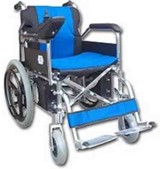
\includegraphics[scale=1]{gambar/kursirodaelektrik.jpg}
  % Keterangan gambar yang diinputkan
  \caption{Kursi Roda Elektrik \parencite{alatkesehatanonline2023}}
  % Label referensi dari gambar yang diinputkan
  \label{fig:metodelogi}
\end{figure}

Kursi roda elektrik memiliki beberapa kategori Berdasarkan karakteristiknya yang mana dapat dijadikan menjadi tiga kategori yaitu:
\begin{enumerate}
    \item Kursi bertenaga roda depan: kursi roda ini biasa dipakai di dalam ruangan. Kursi roda ini merupakan kategori yang yang paling fleksibel.
    \item Kursi bertenaga roda belakang: kursi roda ini biasa dipakai di luar ruangan. Kursi roda ini merupakan cocok dipakai pada jalan kasar.
    \item Kursi roda bertenaga roda tengah: kursi roda ini biasa dipakai di dalam ruangan. Perbedaannya dibandingkan dengan tenaga roda depan adalah fungsi kemudi yang kokoh \parencite{Asnan2019SNI}. 
\end{enumerate}

\subsection{Touchpad}
Touchpad atau bisa disebut bantalan sentuh pertama kali digunakan pada komputer Apollo, sebuah komputer desktop yang dilengkapi dengan touchpad di sisi kanan keyboard “apollo-started”. Touchpad mayoritas digunakan dalam laptop dan memerlukan permukaan yang datar di dekat mesin \parencite{sains_2023}. Touchpad pada laptop biasanya memiliki dua tombol seperti pada mouse. Namun, Semakin dengan perkembangan jangan touchpad sudah tidak lagi diikuti dengan tombol. Hal ini dikarenakan oleh teknologi multi-gesture yang ada pada touchpad.

\begin{figure} [H] \centering
  % Nama dari file gambar yang diinputkan
  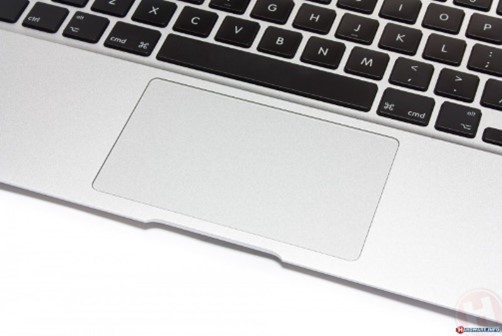
\includegraphics[scale=1]{gambar/Touchpad.jpg}
  % Keterangan gambar yang diinputkan
  \caption{Touchpad pada laptop \parencite{WinPoinPrecisionTouchpad}}
  % Label referensi dari gambar yang diinputkan
  \label{fig:metodelogi}
\end{figure}

Beberapa gerakan yang dapat dilakukan saat menggunakan touchpad adalah sebagai berikut:
\begin{enumerate}
    \item Memilih sesuatu: tekan sekali pada touchpad.
    \item \textit{Scroll}: tekan dan tahan dua jari dan geser secara horizontal atau vertical.
    \item Memperbesar atau memperkecil: taruh dua jari pada touchpad lalu cubit kedalam atau rentangkan.
    \item Menampilkan perintah tambahan: tekan sekali dengan dua jari pada touchpad, atau tekan sekali di kanan bawah touchpad \parencite{MicrosoftTouchGestures}.
\end{enumerate}
Selain Gerakan di atas, masih banyak Gerakan lain yang dapat dilakukan pada touchpad untuk mengoperasikan laptop.

\subsection{Raspberry Pi 4}
Raspberry Pi merupakan komputer papan tunggal atau bisa disebut single-board computer yang seukuran kartu ATM, dikembangkan oleh Raspberry Pi Foundation. Raspberry pi biasanya digunakan pada proyek Internet of Things (IoT). Hal ini dikarenakan raspberry pi berfungsi sebagai komputer papan tunggal yang mampu menjalankan berbagai program, dari penggunaan perkantoran hingga menjadi pemutar media. Raspberry Pi juga memiliki fitur 40-pin GPIO, yang mana dapat digunakan untuk menghubungkan dan mengendalikan berbagai komponen elektronik, hal ini menjadikan raspberry pi sebagai alat yang ideal untuk melakukan eksperimen dan proyek pembelajaran dalam bidang komputasi fisik, pemrograman, dan IoT \parencite{Besari24JamIoT}.

\begin{figure} [H] \centering
  % Nama dari file gambar yang diinputkan
  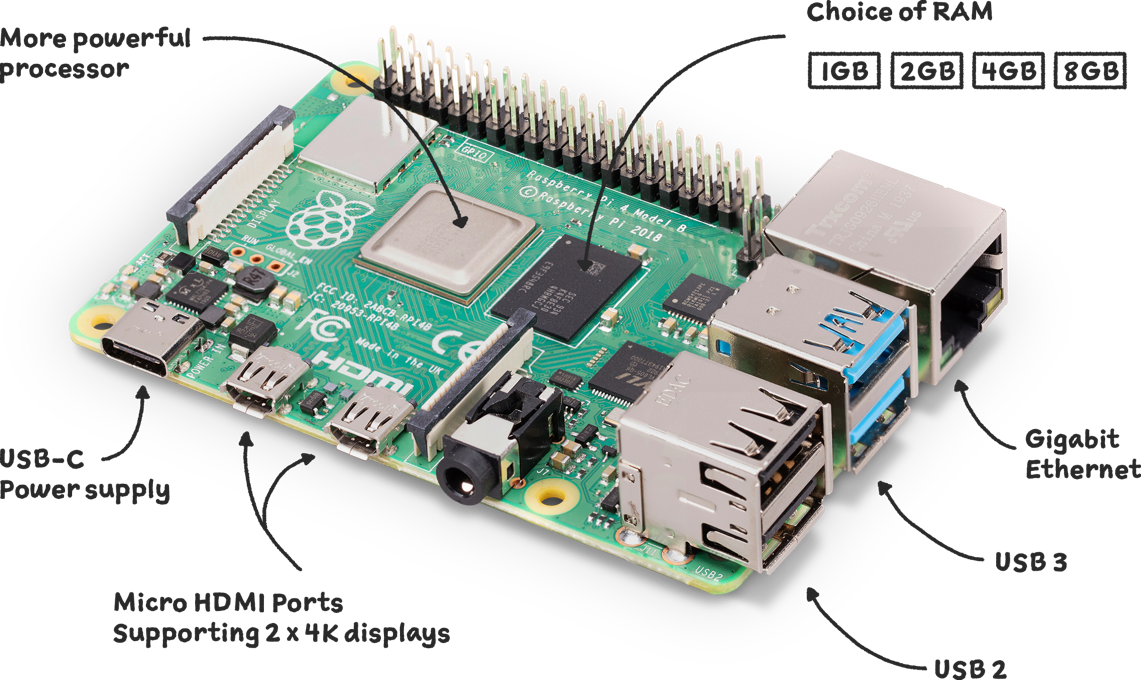
\includegraphics[scale=0.3]{gambar/raspberrypi4.png}
  % Keterangan gambar yang diinputkan
  \caption{Raspberry Pi 4 \parencite{raspberrypiltd_2023}}
  % Label referensi dari gambar yang diinputkan
  \label{fig:metodelogi}
\end{figure}





  \cleardoublepage

  % Konten metodologi
  \chapter{METODOLOGI}

% Ubah konten-konten berikut sesuai dengan isi dari metodologi

\section{Data dan Peralatan}

\textbf{Data}
\begin{enumerate}
    \item Input Toucpad
\end{enumerate}

\textbf{Peralatan}
\begin{enumerate}
    \item Laptop Asus Zenbook 13
    \item Touchpad Wireless 
    \item Kursi Roda Elektrik
    \item Raspberry Pi 4
\end{enumerate}

\section{Metode yang digunakan}
% Dahului dengan gambar Blok Diagram, kemudian pada bagian berikutnya jelaskan masing- masing blok.
% Contoh input gambar dengan format *.jpg
\begin{figure} [H] \centering
  % Nama dari file gambar yang diinputkan
  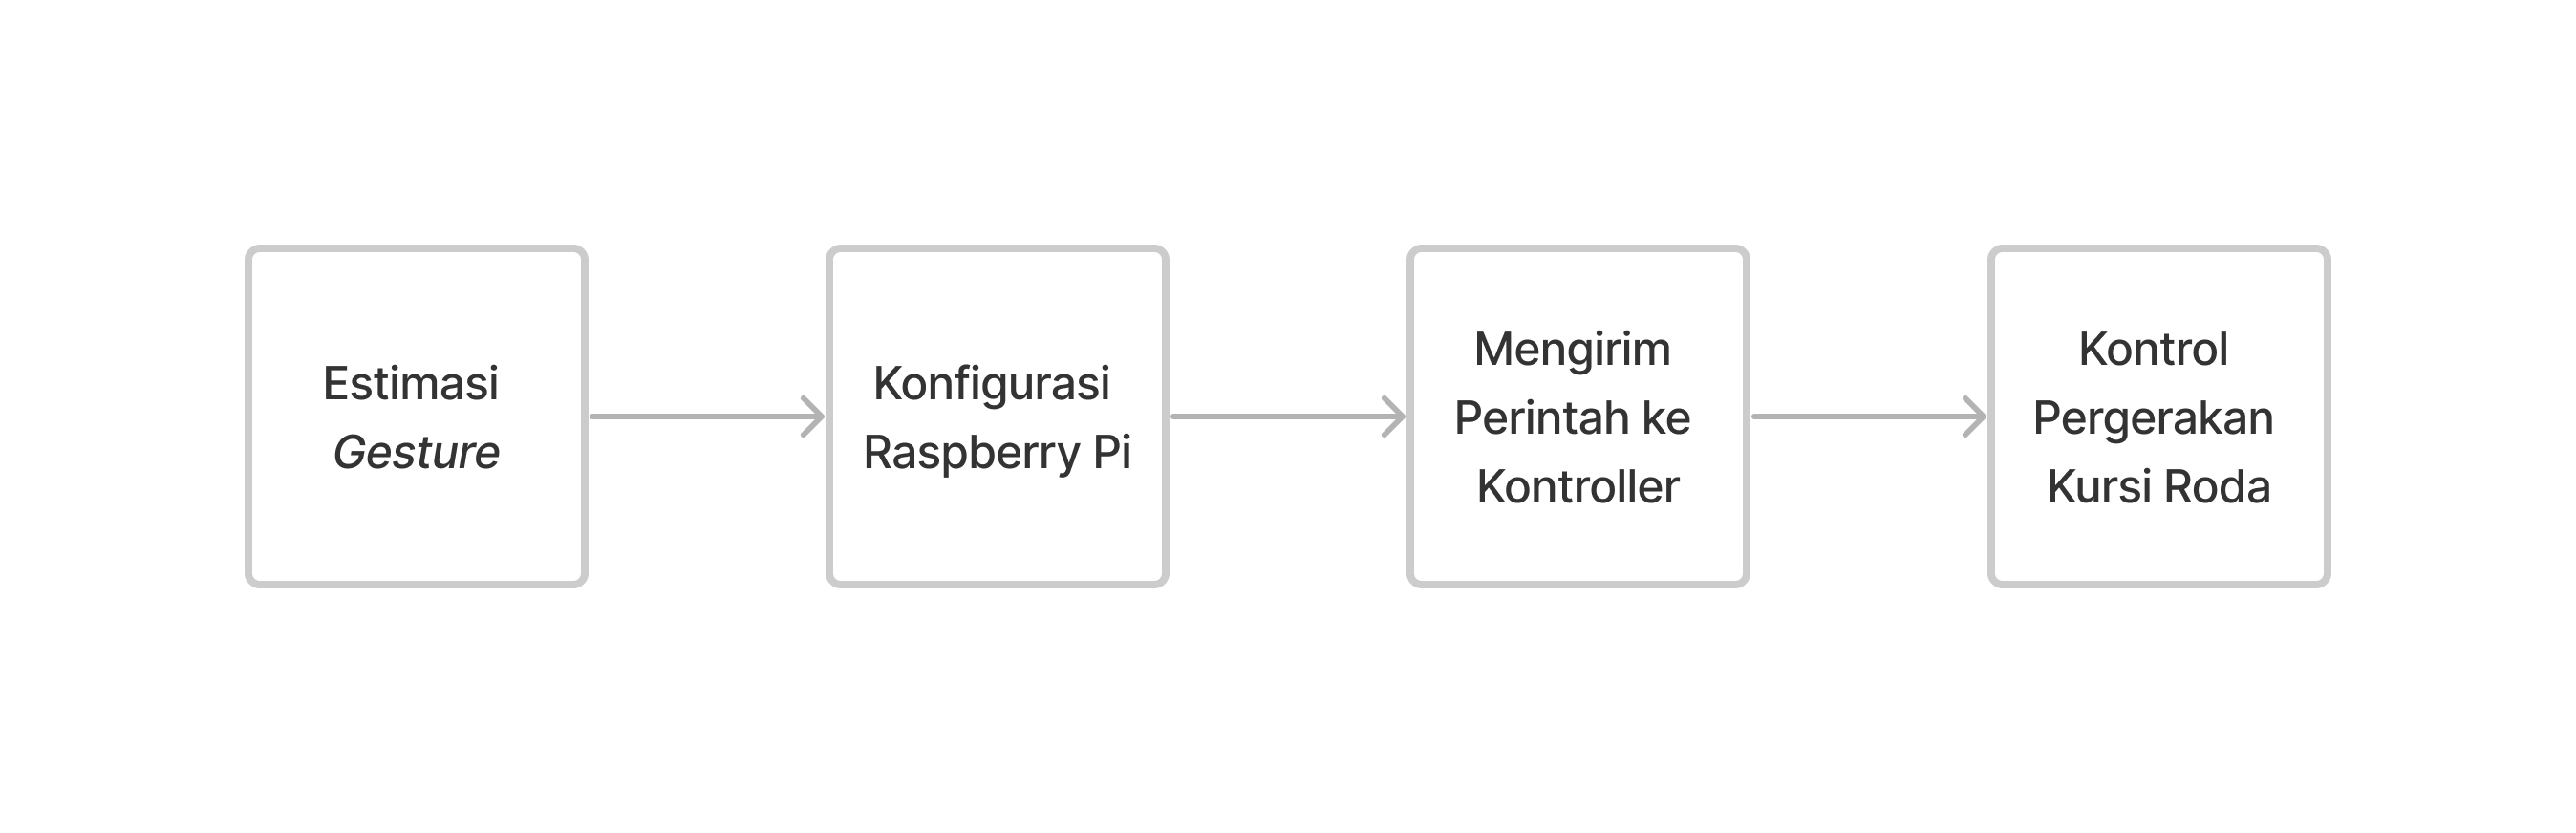
\includegraphics[scale=0.3]{gambar/metodologi.jpg}
  % Keterangan gambar yang diinputkan
  \caption{Metodelogi}
  % Label referensi dari gambar yang diinputkan
  \label{fig:metodelogi}
\end{figure}

% Contoh penggunaan referensi dari gambar yang diinputkan
\subsection{Estimasi Gesture}
Pada bagian ini saya menggunakan touchpad untuk menerima gesture. Saat jari memberikan gesture maka touchpad akan langsung mengestimasi gerakan apa yang diberikan oleh jari. setelah touchpad tau gerakan apa yang diberikan, output akan dikirimkan kepada Raspberry pi untuk diklasifikasi.

\subsection{Konfigurasi Raspberry Pi}
Disini saya memilih untuk menggunakan Raspberry Pi sebagai kepala dari rangkaian penelitian ini. pada raspberry pi dilakukan konfigurasi agar dapat mengklasifikasikan gesture apa yang diberikan oleh touchpad. Setelah dilakukan konfigurasi berdasarkan tiap-tiap gesture, maka akan dikirim data kepada kontroller

\subsection{Kontrol Pergerakan Kursi Roda}
Setelah kontroller menerima data dari raspberry pi, data tersebut langsung di jalankan sehingga kursi roda akan bergerak berdasarkan data yang telah diklasifikasikan oleh raspberry pi

% Pada \emph Blok Diagram \ref{fig:metodelogi}. Dapat dilihat bahwa pertama adalah mengestimasi gesture yang diberikan kepada touchpad. Setelah diestimasi maka raspberry pi akan melakukan konfigurasi dari gesture yang diberikan. setelah itu raspberry pi akan mengirimkan perintah ke kontroller karena gesture sudah di terkonfigurasi. kursi roda akan bergerak sesuai dengan perintah yang dikirim oleh raspberry pi


  \cleardoublepage

  % Konten lainnya
  \chapter{HASIL}

\section{Hasil yang Diharapkan}

Hasil yang diharapkan dari keberhasilan pengembangan sistem ini adalah pengguna kursi roda elektrik akan mendapatkan sistem kendali yang kuat dan juga tahan lama dibandingkan dengan sistem kendali \textit{joystick}.

\section{Hasil Pendahuluan}

Sampai saat ini, saya telah mencoba untuk menggunakan \textit{touchpad} \textit{wireless} kepada laptop, dan sudah dipastikan bahwa \textit{touchpad} tersebut dapat berfungsi dengan baik. Selain itu, kursi roda sudah dipasangi dengan \textit{Motor Driver}. 

  \cleardoublepage

  % Konten jadwal penelitian
      \chapter{JADWAL PENELITIAN}

% Ubah tabel berikut sesuai dengan isi dari rencana kerja
\newcommand{\w}{}
\newcommand{\G}{\cellcolor{gray}}
\newcommand{\B}{\cellcolor{blue}}
\begin{table}[H]
  \captionof{table}{Tabel timeline}
  \label{tbl:timeline}
  \begin{tabular}{|p{3.5cm}|c|c|c|c|c|c|c|c|c|c|c|c|c|c|c|c|}

    \hline
    \multirow{2}{*}{Kegiatan} & \multicolumn{16}{|c|}{Minggu}                                                                       \\
    \cline{2-17}              &
    1                         & 2                             & 3  & 4  & 5  & 6  & 7  & 8  & 9  & 10 & 11 & 12 & 13 & 14 & 15 & 16 \\
    \hline

    % Gunakan \G untuk mengisi sel dan \w untuk mengosongkan sel
    Studi literasi          &
    \G                        & \G                            & \G & \G & \w & \w & \w & \w & \w & \w & \w & \w & \w & \w & \w & \w \\
    \hline

    Perancangan dan desain sistem kendali           &
    \w                        & \w                            & \w & \w & \G & \G & \G & \G & \w & \w & \w & \w & \w & \w & \w & \w \\
    \hline

    Perakitan dan pemasangan pada kursi roda              &
    \w                        & \w                            & \w & \w & \w & \w & \w & \w & \G & \G & \G & \G & \w & \w & \w & \w \\
    \hline

    Pengujian alat dan evaluasi hasil       &
    \w                        & \w                            & \w & \w & \w & \w & \w & \w & \w & \w & \w & \w & \G & \G & \G & \G \\
    \hline
  \end{tabular}
\end{table}

Pada \emph{timeline} yang tertera di Tabel \ref{tbl:timeline}, pada empat minggu pertama dilakukan studi literasi terdahulu mengenai apa saja yang ada di dasar teori. Setelah melakukan studi literasi, dilakukan perancangan dan desain sistem kendali. mulai dari bagaimana pemasangan \textit{raspberry pi} pada kursi roda, perkabelan rangkaian, dan peletakan \textit{touchpad} pada kursi roda. Setelah merancang dan mendesain semua dengan baik, dimulailah perakitan dan pemasangan semua alat kepada kursi roda. yang terakhir adalah melakukan uji coba alat dan mengevaluasi hasil dari uji coba alat tersebut. 


  \cleardoublepage


  % Daftar pustaka
  \chapter*{DAFTAR PUSTAKA}
  \addcontentsline{toc}{chapter}{DAFTAR PUSTAKA}
  \renewcommand\refname{}
  \vspace{2ex}
  \renewcommand{\bibname}{}
  \begingroup
    \def\chapter*#1{}
    \printbibliography
  \endgroup


\end{document}
